\documentclass[tikz]{standalone}

\usepackage{fontspec}

\usetikzlibrary{arrows}
\usetikzlibrary{calc}
\usetikzlibrary{decorations.pathreplacing}
\usetikzlibrary{positioning}
\usetikzlibrary{matrix}

\usepackage{fontspec}

\begin{document}

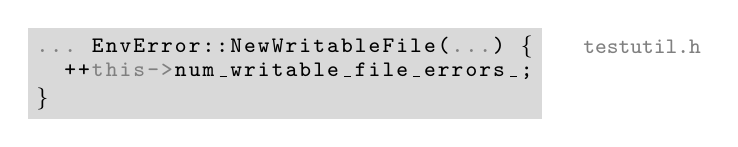
\begin{tikzpicture}
  [node distance=5mm, >=stealth',
  every node/.style={font=\footnotesize},
  every matrix/.style={fill=black!15, inner sep=1mm, row sep=0.5mm,
                        matrix of nodes, nodes in empty cells,
                        minimum height=0.5em, minimum width=.5em,
                        nodes={anchor=base, inner sep=0, font=\ttfamily\footnotesize}}]

  \matrix (snippet) {
|[black!50]|. & |[black!50]|. & |[black!50]|. &   & E & n & v & E & r & r & o & r & : & : & N & e & w & W & r & i & t & a & b & l & e & F & i & l & e & ( & |[black!50]|. & |[black!50]|. & |[black!50]|. & ) &   & \{ \\
  &   & + & + & |[black!50]|t & |[black!50]|h & |[black!50]|i & |[black!50]|s & |[black!50]|- & |[black!50]|> & n & u & m & \_ & w & r & i & t & a & b & l & e & \_ & f & i & l & e & \_ & e & r & r & o & r & s & \_ & ; \\
\} &   &   &   &   &   &   &   &   &   &   &   &   &   &   &   &   &   &   &   &   &   &   &   &   &   &   &   &   &   &   &   &   &   &   &   \\
  };

 \node [above, anchor=west, black!50, xshift=0.5cm]
        at (snippet-1-36.east)
        {\texttt{testutil.h}};
\end{tikzpicture}

\end{document}
